\documentclass[9pt,a4paper]{report}
\usepackage{mwe}
\usepackage{listings}
\usepackage{amsmath}
\usepackage{graphicx}
\usepackage{subfig}
\usepackage{float}
\usepackage{xcolor}
\usepackage{multirow}
\usepackage{hyperref}
\usepackage{fancyhdr}
\usepackage{sectsty}
\usepackage[dvipsnames]{xcolor}
\usepackage{soul}
\usepackage[compact]{titlesec}
\usepackage{float}
\usepackage[left=0.5cm,right=0.5cm,top=0.5cm,bottom=0.5cm]{geometry}
\graphicspath{}

\newcommand*{\nchapter}[1]{%
	\chapter*{#1}%
	\addcontentsline{toc}{chapter}{#1}
	\vspace{-14mm}}
\newcommand*{\nsection}[1]{%
	\section*{#1}%
	\addcontentsline{toc}{section}{#1}}
\newcommand*{\nsubsection}[1]{%
	\subsection*{#1}%
	\addcontentsline{toc}{subsection}{#1}}
\newcommand*{\nsubsubsection}[1]{%
	\subsubsection*{#1}%
	\addcontentsline{toc}{subsubsection}{#1}}

\chaptertitlefont{\large}
\sectionfont{\normalsize}
\fontsize{9}{11}\selectfont
\begin{document}
	\begin{titlepage}
		\centering
		\vspace*{1.5in}
		
\includegraphics[width=0.15\textwidth]{W-Logo_Purple_RGB}\par\vspace{1cm}
		{\LARGE \textsc{University of Washington}\par}
		\vspace{1cm}
		{\Large \textsc{BEE331 Lab 4}\par}
		\vspace{1.5cm}
		{\huge\bfseries \par}
		\vspace{2cm}
		{\Large\itshape 2301991\hspace{55pt}2130474\par}
		{\Large\itshape Jason Truong\hspace{31pt}Henry Haight\par}
		\vfill
		supervised by\par
		Prof.~Joseph \textsc{Decuir}
		\date{2024\\ January}
		\vfill
		% Bottom of the page
		{\large \today\par}
		\vspace*{1.5in}
	\end{titlepage}
	
	\nchapter{NMOS Amplifier Circuit}
	\nsection{Design Objective}
	In this lab, we introduce ourselves to the MOSFET Amplifier. We characterise and build an audio-amplifier's small-signal single-stage circuit.
	\begingroup
	\renewcommand{\cleardoublepage}{}
	\renewcommand{\clearpage}{}
	\nsection{Circuit Design Outline}
	\endgroup
	With a sinusoidal voltage source $V_{AC}$ - @ $V_p=50mV$ and a frequency of $10kHz$ in series with a capacitor $C_{C1}=0.1\mu F$. In parallel - a series DC voltage source $V_{DD}$ connected to a resistor $R_{G_1}=38.2k$, another resistor $R_{G_2}=95.3k$, and Gate to an NMOSFET $NMOS_G$.\\
	From the NMOSFET,
	\begin{itemize}
		\item Source
		\subitem Parallel, a capacitor $C_s = 10\mu F$ and resistor $R_S=200\Omega$.
		\item Drain
		\subitem In parallel - a resistor $R_D = 500\Omega$, to a series Capacitor $C_{C2}$ and Resistor $R_L$.
	\end{itemize}
	\newpage
	\nsection{Descriptions of Measurements \& Calculations}
	\nsubsection{Analysis}
	\begin{itemize}
		\item \textbf{1.2.3 Calculate the Voltage gain of the amplifier circuit of Figure 6 using the following two equations:}
		\subitem $\frac{v_o}{v_{sig}=g_mR_d}$
		\subitem $g_m=k_nV_{ov}=\frac{2I_D}{V_{ov}}$
		
		\item \textbf{2.3 How does the calculated voltage gain (using $\frac{v_o}{v_{sig}}=g_mR_D$) compare with the measured voltage gain? Explain the potential sources of error. You can reference your explanation to the more previse expression for the voltage gain.}
		\subitem How does the calculate Voltage Gain compare?
		\subsubitem See addendum for calculations
		
		\subitem Sources of Error
		\subsubitem Imperfect Components
		\subsubitem Imprecise Calculations (approximates)
		\subsubitem Metrics of $R_D$ leading to a lowered measured gain.
		\subsubitem Measurements error overall.
		
		\item \textbf{2.4 Give a brief summary of how your audio amplifier worked and what gain in decibels ($|A_v|_{dB}=20log(\frac{v_o}{v_{sig}})$ you achieved at 10 kHz)}
		\subitem [See addendum for calculations]
		\subitem The audio amplifier's output is dependent on the ratio of $\frac{v_o}{v_{sig}}$.
		
		\item \textbf{2.5 How would you increase the gain by an additional 10 dB? How does the gain behave as a function of frequency?}
		\subitem [See addendum for calculations]
		\subitem Understand voltage gain in dB $20log\approx3.16$
		\subsubitem $A_v^new=3.16*A_v^{original}$
		\subsubitem Increasing the value of the Midband $g_mR_D$
		\subsubitem Decreasing the High-Frequency Roll-Off in the MOSFET
		\subitem Gain behaves as a function of frequency in relation to $v_{sig}=V_pcos(2\pi f+\phi)$.
	\end{itemize}
	\begin{figure}[hp!] %140, 
		\centering
		\caption{MOSFET Amplifier}
		\subfloat[\centering NMOS Amplifier]{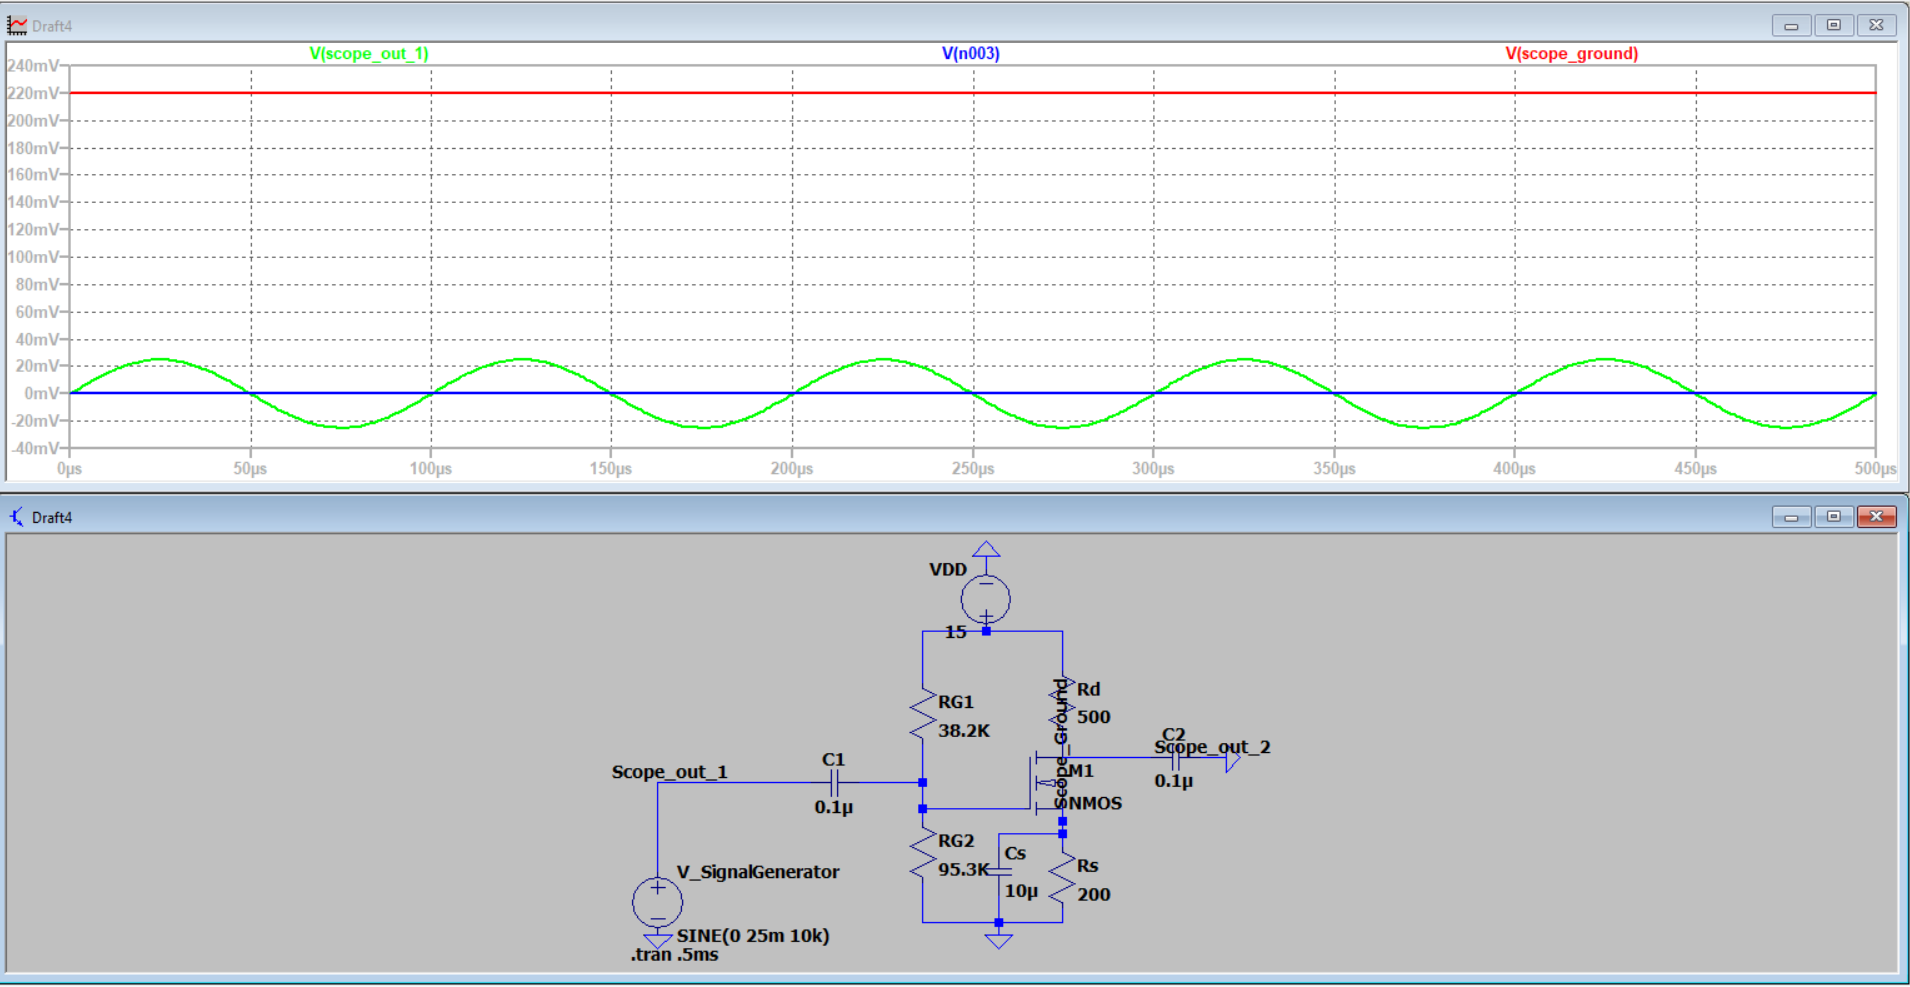
\includegraphics[width=9cm]{Lab4-2 screenshot}}\hfil
		\subfloat[\centering Oscilloscope Measurements]{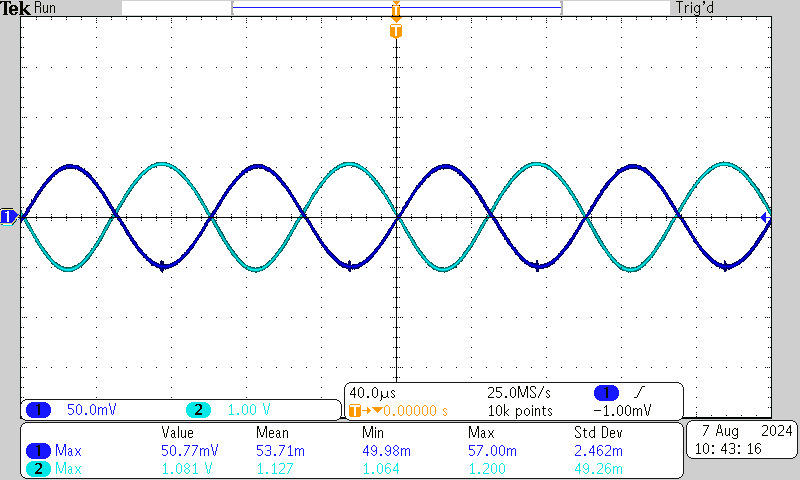
\includegraphics[width=9cm]{tek0001}}
	\end{figure}
	
	\nsection{Summary \& Conclusions}
	Revealed in Figure RD-Circuit 1A \& 1B, the generated oscilloscope readings of the two periodic function match the characteristics of the transfer function found in  1b (RD Circuit). So the measurements do infact closely align.
	
	\newpage
	\nchapter{Addendum Pages}
	\begin{figure}[hp!]
		\centering
		\caption{Jason Truong Addendum}
		\subfloat[Lab 4 Calculations\centering]{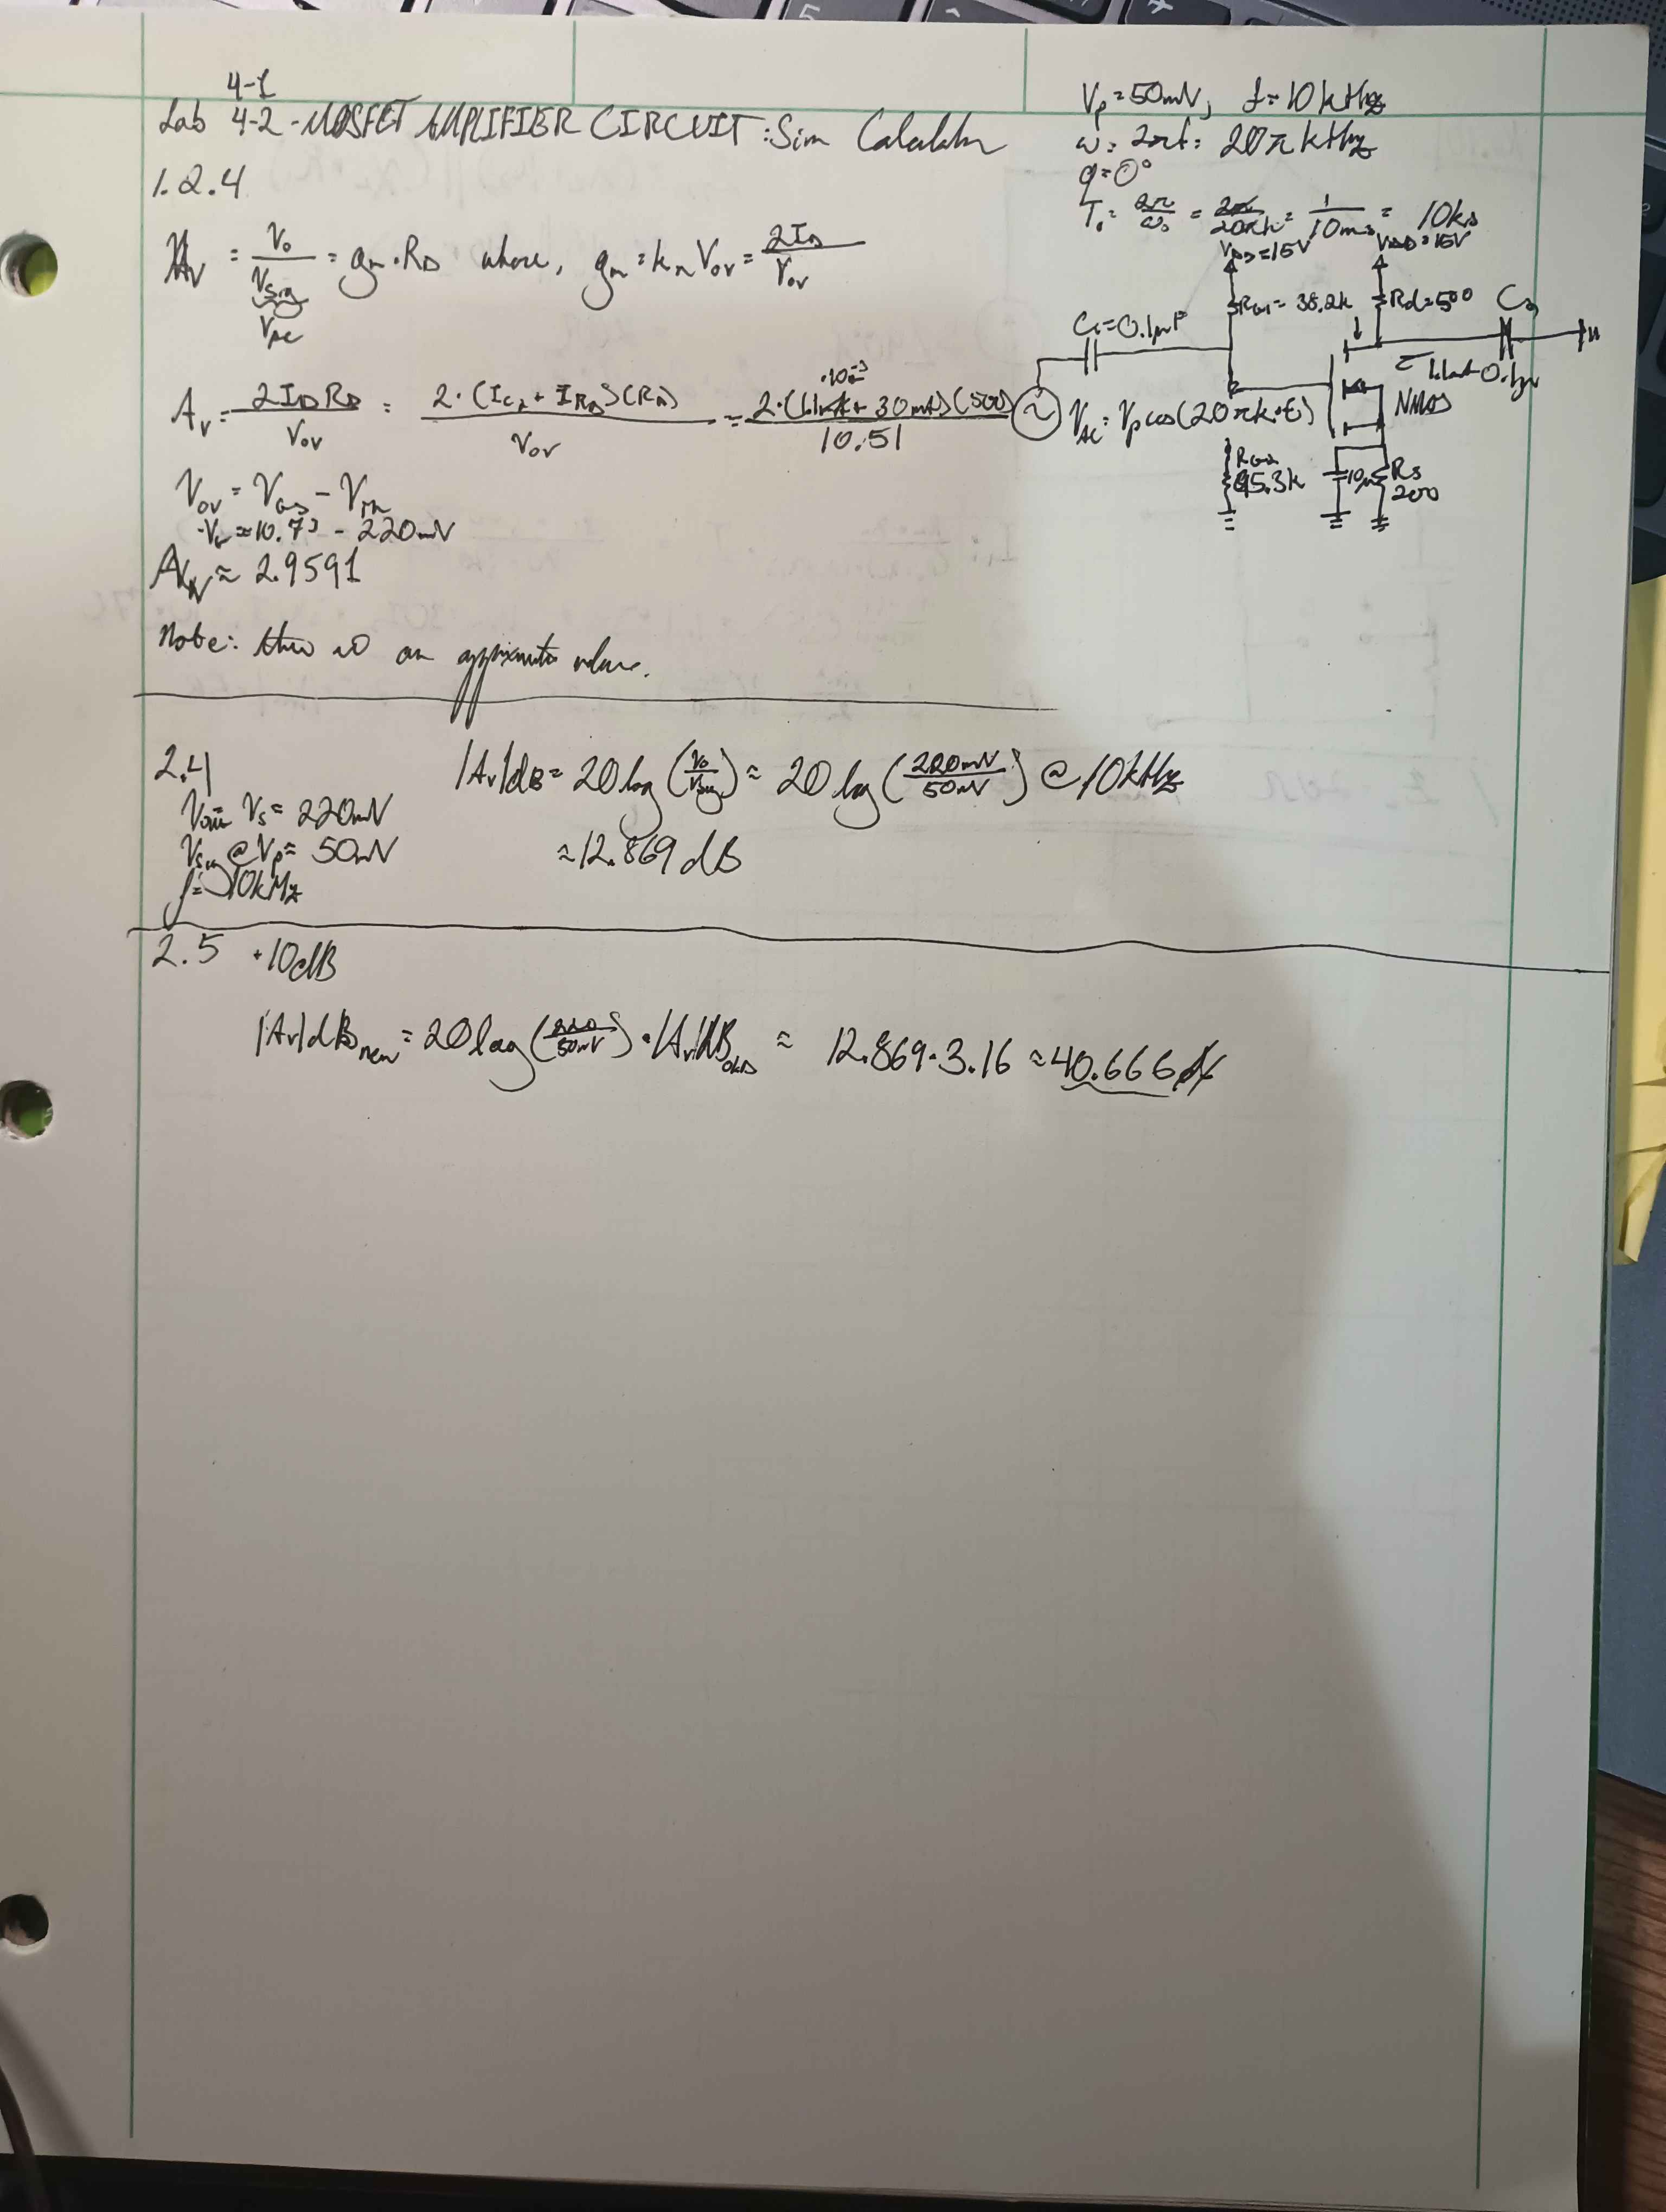
\includegraphics[width=15cm]{IMG_20240809_055234116}}
	\end{figure}
	\nsection{Bibliography}
	\textbf{Cited:}\\
	\begin{itemize}
		\item Lab 1 Manual
		\item Sedra, Adel, and Kenneth Smith. Microelectronic Circuits. S.L., Oxford Univ Press Us, 2019.
		\item “How Do You Calculate, a Silicon Junction Diode with N = 1 Has v = 0.7 v al I = 1 MA. What Is the Voltage Drop at I=0.1 MA and I=10 MA.?” Quora, 2024, appliedmathematics.quora.com/How-to-calculate-A-silicon-junction-diode-with-n-1-has-v-0-7-V-al-I-1-mA-What-is-the-voltage-drop-at-I-0-1-mA-an?top\_ans=223007030. Accessed 15 July 2024.
	\end{itemize}
	\begin{figure}[!h]
		\centering
		\subfloat[Good work.\centering]{
\includegraphics[width=15cm]{Yusa}}
	\end{figure}
\end{document}